\section{Construction of Topologies} 

  \subsection{Subspace Topologies} 

    \begin{theorem}[Subspace Topology]
      Given topological space $X$ and subspace $Y \subset X$, the topology of $X$ induces the topology of $Y$ in the following way. 
      \begin{equation}
        \T_Y = \{(U \cap Y) \subset Y \;|\; U \in \T_X\}
      \end{equation}
      That is, the open sets of $Y$ are defined to be the intersection of the open sets of $X$ with the space $Y$. This is called the \textbf{subspace topology}. 
    \end{theorem} 
    \begin{proof}
      We prove the properties. 
      \begin{enumerate}
        \item \textit{Trivial}. We see that $\emptyset = \emptyset \cap Y$ and $Y = X \cap Y$. 
        \item \textit{Stability under Union}. Suppose $\{V_\alpha\}_{\alpha \in A}$ are setes that are open in $Y$. Then for each $\alpha$ there exists an open set $U_\alpha \subset X$ that is open in $X$. Therefore, 
        \begin{align}
          \bigcup_{\alpha \in A} V_\alpha & = \bigcup_{\alpha \in A} (U_\alpha \cap Y) \\ 
                                          & = Y \cap \bigg( \bigcup_{\alpha \in A} U_\alpha \bigg)
        \end{align}
        where $\cup_\alpha U_\alpha$ is open in $X$, and therefore we shown that there exists such an open set. 

        \item \textit{Stability under Finite Intersection}. Suppose $\{V_i\}_{i = 1}^n$ are open in $Y$. Then we can do the same thing. 
      \end{enumerate}
    \end{proof}

    The reason we want to do this is because we want to think of $Y$ as its own entity, independent of $X$. 

    \begin{figure}[H]
      \centering 
      \includegraphics[scale=0.25]{img/Subspace_Topology.PNG}
      \caption{The subspace topology of a line $l$ embedded in $\mathbb{R}^2$ and that of a surface $\mathcal{L}$ embedded in $\mathbb{R}^3$ is shown.}
      \label{fig:subspace_topology}
    \end{figure} 

    \begin{example}[Non-Open Sets may be Open in Subspace]
      Let $X = \mathbb{R}$ with the Euclidean topology and let $Y = [0, 1]$. 
      \begin{enumerate}
        \item $[0, 1]$ is open in $Y$ but not in $X$. 
        \item Intervals of the form $(a, 1]$ and $[0, b)$ are open in $Y$ but not in $X$. 
      \end{enumerate}
    \end{example} 

    \begin{example}[Singleton Sets in Subspace Topologies]
      Consider $X = \mathbb{R}$ with the lower limit topology with $Y = [0, 1]$. The following 
      \begin{enumerate}
        \item $[1/2, 1] = Y \cap [1/2, 2)$, and 
        \item $\{1\} = Y \cap [1, 2)$
      \end{enumerate}
      are open in the subspace topology. It turns out that $\{1\}$ is the only singleton set open in $Y$. 
    \end{example}

    Consider any set $U \subset Y$. Note that if $U$ is an open set in $X$ that happens to be contained in $Y$, then we can set $U = U \cap Y$, so $U$ is open in $Y$. However, we have seen that being open in $Y$ does not necessarily imply that it is open in $X$. 

    \begin{theorem}[Induced Basis of Subspace Topologies]
      If $\B$ is a basis for the topology of $X$, then 
      \begin{equation}
        \B_Y \coloneqq \{B \cap Y \mid B \in \B \} 
      \end{equation}
      is a basis for the subspace topology of $Y$. 
    \end{theorem}
    \begin{proof}
      
    \end{proof}

    \begin{example}[Induced Basis]
      The basis for the subspace topology of $[0, 1] \subset \mathbb{R}$ with the Euclidean topology consists of the intervals 
      \begin{enumerate}
        \item $(a, b)$ where $0 \leq a < b \leq 1$. 
        \item $[0, b)$ where $0 < b \leq 1$. 
        \item $(a, 1]$ where $0 \leq a < 1$. 
      \end{enumerate}
    \end{example} 

    \begin{example}[Unit Sphere]
      Let $S^n \subset \mathbb{R}^{n+1}$ be the unit \textbf{n-sphere} defined 
      \begin{equation}
        S^n \coloneqq \{x \in \mathbb{R}^{n+1} \mid ||x||^2 = 1 \}
      \end{equation}
      When thinking about $S^n$ as a space itself, we use the subspace topology coming from the standard topology of $\mathbb{R}^n$. 
    \end{example}

    Let's focus on $n = 1$. For $a < b$, let 
    \begin{equation}
      A_{a, b} = \{ (\cos{t}, \sin{t}) \mid a < t < b \}
    \end{equation} 
    Then, we can see that
    \begin{enumerate}
      \item if $b - a > 2 \pi$, then $A_{a, b} = S^1$. 
      \item If $b - a \leq 2 \pi$, then $A_{a, b}$ is an ``open arc'' from $(\cos{a}, \sin{a})$ to $(\cos{b}, \sin{b})$.  
    \end{enumerate} 

    \begin{theorem}[Basis for $S^1$]
      Given that we have an equivalence class defined 
      \begin{equation}
        A_{a, b} \sim A_{a + 2 \pi k, b + 2 \pi k} \text{ for all } k \in \mathbb{Z}
      \end{equation} 
      We claim that $\{A_{a, b}\}$ is a basis for the subspace topology of $S^1$. 
    \end{theorem} 
    \begin{proof}
      
    \end{proof}

    \begin{example}
      We can see that the open arc covering the top right quadrant in $\mathbb{R}^2$ is 
      \begin{equation}
        S^1 \cap (0, 1)^2 = S^1 \cap B_\infty \big( (\frac{1}{2}, \frac{1}{2}), \frac{1}{2} \big)
      \end{equation}
    \end{example} 

    Now let's focus more on metric spaces. Note that if we want to construct topologies of subspaces of metric spaces, there are two ways to do it. It would be quite bad if these resulted in different topologies, but fortunately we have the following theorem. 

    \begin{theorem}[Topologies on Subspaces of Metric Spaces Coincide]
      Let $(X, d_X)$ be a metric space, with $Y \subset X$. There are 2 ways we can define a topology on $Y$. 
      \begin{enumerate}
        \item Take the metric topology $\T_X$ on $X$, and then take the subspace topology on $Y$. 
        \item Induce a metric $d_Y = d_{X | Y}$ on $Y$ which is a restriction of $d_X$ to $Y$, and then take the metric topology of it. 
      \end{enumerate}
      We claim that these two constructions give the same topology, as shown in the commutative diagram. 

      \begin{figure}[H]
        \centering 
        \begin{tikzcd}
          d_X \arrow[r] \arrow[d] & d_Y \arrow[d] \\
          \T_X \arrow[r] & \T_Y 
        \end{tikzcd}
        \caption{} 
        \label{fig:same_construction}
      \end{figure}
    \end{theorem}
    \begin{proof}
      The basis for the subspace topology on $Y$ is 
      \begin{equation}
        \B_1 = \{B_{d_X} (x, r) \cap Y \mid x \in X, r > 0 \}
      \end{equation} 
      and the basis for the (induced) metric topology on $Y$ is 
      \begin{equation}
        \B_2 = \{B_{d_Y} (y, r) \cap Y \mid y \in Y, r > 0 \} = \{B_{d_X} (y, r) \cap Y \mid y \in Y, r > 0 \}
      \end{equation} 
      It is immediate that $\B_2 \subset \B_1$ since it goes over all $x \in X$ rather than $y \in Y$. To see why $\B_1 \subset \B_2$, TBD. 
    \end{proof}


  \subsection{Box and Product Topologies} 

    There are multiple ways to define the box and product topologies, but their construction with basis elements is most simple. 

    \begin{theorem}[Box Topology]
      Let $\{X_\alpha\}_{\alpha \in I}$ be an indexed (finite or countably infinite) family of topological spaces and let us take the product of these spaces
      \begin{equation}
        \prod_{\alpha \in I} X_\alpha
      \end{equation}
      We could endow the \textbf{box topology} of all open sets in the form
      \begin{equation}
        \prod_{\alpha \in I} U_\alpha
      \end{equation}
      where $U_\alpha$ is open in $X_\alpha$ for each $\alpha \in I$. It is clear that a basis element $B$ of the box topology is of form
      \begin{equation}
        B = \prod_{\alpha \in I} B_\alpha
      \end{equation}
      where $B_\alpha$ is a basis element of the topology of each component space $X_\alpha$. 
      \begin{figure}[H]
        \centering 
        \begin{tikzpicture}
          \draw[<->] (-1,0)--(6,0);
          \draw[<->] (0,-1)--(0,4);
          \draw[dashed] (1,1)--(1,3)--(4,3)--(4,1)--(1,1);
          \node[below] at (6,0) {$\mathbb{R}$};
          \node[left] at (0,4) {$\mathbb{R}$};
          \node[below] at (1,-0.3) {$a$};
          \node[below] at (4,-0.3) {$b$};
          \node[left] at (-0.3,1) {$c$};
          \node[left] at (-0.3,3) {$d$};
          \node[rotate=90] at (0,1) {$($};
          \node[rotate=-90] at (0,3) {$($};
          \node at (1,0) {$($};
          \node at (4,0) {$)$};
        \end{tikzpicture}
        \caption{We can visualize the elements of the box topology with the product space $\mathbb{R}^2 = \mathbb{R} \times \mathbb{R}$, where each $\mathbb{R}$ has an open ball topology. From the visual below, we can see why this is called the "box" topology. Furthermore, all basis elements of this space are arbitrary open rectangles in $\mathbb{R}^2$. }
        \label{fig:box_topology}
      \end{figure}
    \end{theorem}
    \begin{proof}
      It is easy to prove that the box topology indeed satisfies the 3 properties of topologies in general. 
    \end{proof}

    While this topology may seem quite "intuitive" for the first learner, the box topology, however, has serious limitations when extending to infinite Cartesian products of spaces. Let 
    \begin{equation}
      \pi_\beta: \prod_{\alpha \in I} X_\alpha \longrightarrow X_\beta, \; \pi_\beta \big( (x_\alpha)_{\alpha \in I}\big) \equiv x_\beta\
    \end{equation}
    be the projection mapping of an element in the product space to the $\beta$th space. 

    \begin{theorem}[Product Topology]
      Let $\{X_\alpha\}_{\alpha \in I}$ be an indexed family of topological spaces with their product space defined as above. Given an open set $U_\beta \subset X_\beta$, let us define $\mathscr{S} (U_\beta) \subset \prod X_\alpha$ as 
      \begin{equation}
        \mathscr{S}(U_\beta) \equiv X_1 \times X_2 \times ... \times X_{\beta -1} \times U_\beta \times X_{\beta+1} \times ... 
      \end{equation}
      \begin{figure}[H]
        \centering 
        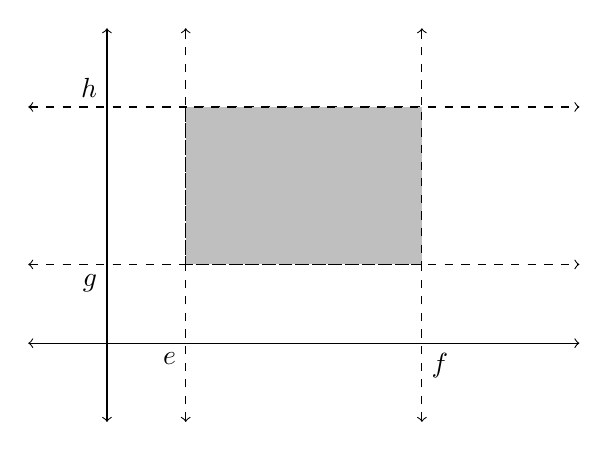
\begin{tikzpicture}
          \draw[<->] (-1,0)--(6,0);
          \draw[<->] (0,-1)--(0,4);
          \draw[<->, dashed] (-1,1)--(6,1);
          \draw[<->, dashed] (-1,3)--(6,3);
          \draw[<->, dashed] (1,-1)--(1,4);
          \draw[<->, dashed] (4,-1)--(4,4);
          \node [below left] at (1,0) {$e$};
          \node [below right] at (4,0) {$f$};
          \node [above left] at (0,3) {$h$};
          \node [below left] at (0,1) {$g$};
          \draw[dashed, fill=lightgray] (1,1) rectangle (4,3);
        \end{tikzpicture}
        \caption{Visually, we can interpret each $\mathscr{S} (U_\beta)$ as a "strip" in the total product space. For example in $\mathbb{R}^2$, there are two "strips" $(e, f) \times \mathbb{R}$ and $\mathbb{R} \times (g, h)$ that intersect. }
        \label{fig:product_topology}
      \end{figure}
      The topology generated by this basis is called the \textbf{product topology}. Note that by the properties of topologies, we can create open sets by taking unions and finite intersections of these basis elements. This means that every open set in the product topology has form
      \begin{equation}
        \prod_{\alpha \in I} U_\alpha
      \end{equation}
      where $U_\alpha$ is an open subset of $X_\alpha$ for finitely many $\alpha$'s and $U_\alpha = X_\alpha$ for the rest. 
    \end{theorem}

    We can deduce some conclusions comparing these topologies. First, the product and box topologies are precisely the same if we work in finite Cartesian products of spaces, since any element of the box topology (left hand side) can be expressed as a finite intersection of some open sets (in the right hand side). That is, if $\text{card}\,I < \infty$, then 
    \[\prod_{\alpha \in I} U_i = \bigcap_{\alpha \in I} \big\{ \prod_{\gamma \in I} W_\gamma \; | \; W_\gamma = U_\gamma \text{ if } \gamma = \alpha, \, W_\gamma = X_\gamma \text{ if } \gamma \neq \alpha\big\}\]
    Secondly, we can see that the box topology is finer than the product topology (strictly finer if working in infinite product spaces). 

    \begin{example}
      The set $(0,1)^\mathbb{N} \subset \mathbb{R}^\mathbb{N}$ is clearly open in the box topology, but it is considered "too tight" to be in the product topology. However, 
      \begin{equation}
        (0,1) \times \mathbb{R} \times \mathbb{R} \times \ldots
      \end{equation}
      is open in the product topology since only one (a finite amount) of the factors is not the whole space. 
    \end{example}

    The main difference between the construction of open sets in the box topology vs the product topology is that the box topology merely describes open sets as direct products of open sets from each coordinate space. That is,
    \begin{equation}
      U_\alpha \text{ open in } X_\alpha \implies \prod_{\alpha \in I} U_\alpha \text{ open in } \prod_{\alpha \in I} X_\alpha
    \end{equation}
    On the other hand, the construction of the product topology is completely dependent on the construction of the projection mappings 
    \begin{equation}
      \pi_\beta: \prod_{\alpha \in I} X_\alpha \longrightarrow X_\beta
    \end{equation}
    to be continuous (and nothing more) so that (by definition) the preimages of open sets in $X_\beta$ under $\pi_\beta$ are open sets in $\prod X_\alpha$. Therefore, the construction of the continuous $\pi_\beta$'s canonically constructs a basis of open sets in $\prod X_\alpha$. Taking the union and finite intersection of these open sets gives us the product topology. 

    \begin{theorem}
      If each space $X_\alpha$ is a Hausdorff space, then 
      \begin{equation}
        \prod_{\alpha} X_\alpha
      \end{equation}
      is also Hausdorff in both the box and product topologies. 
    \end{theorem}

    The following theorem reveals why the product topology is superior than the box topology in product spaces. 

    \begin{theorem}
      Given the function 
      \begin{equation}
        f: A \longrightarrow \prod_{\alpha \in I} X_\alpha, \; f(a) \equiv \big( f_\alpha (a) \big)_{\alpha \in I}
      \end{equation}
      with its component functions $f_\alpha: A \longrightarrow X_\alpha$. Let $\prod X_\alpha$ have the product topology. Then the function $f$ is continuous if and only if each function $f_\alpha$ is continuous. 
    \end{theorem}
    \begin{proof}
      Let $\pi_\beta$ be the projection of this product onto the $\beta$th component space. By construction $\pi_\beta$ is continuous $\implies \pi_\beta^{-1} (U_\beta)$ is a basis element of the product topology of $\prod X_\alpha$. \\
      $(\rightarrow)$ $f$ is continuous, so $f_\beta \equiv \pi_\beta \circ f$, as the composition of continuous functions, is also continuous. \\
      $(\leftarrow)$ Assume that each $f_\beta$ is continuous. Let there be an open set $U_\beta \subset X_\beta$. Then, the canonical open set $\pi_\beta^{-1}$ in the product space $\prod X_\alpha$ is also open. Now, the preimage of $\pi_\beta^{-1} (U_\beta)$ under $f$ is 
      \begin{align*}
        f^{-1} \big( \pi_\beta^{-1} (U_\beta)\big) & = (f^{-1} \circ \pi_\beta^{-1})(U_\beta) \\
        & = (\pi_\beta \circ f)^{-1} (U_\beta) \\
        & = f_\beta^{-1} (U_\beta)
      \end{align*}
      Since $f_\beta$ is already assumed to be continuous, $f_\beta^{-1} (U_\beta)$ is open in $A$. 
    \end{proof}

    This theorem also works for the box topology only if we are working with finite product spaces. But in general, this theorem fails for the box topology. Consider the following example. 

    \begin{example}
    Let $\mathbb{R}^\omega$ be the countably infinite product of $\mathbb{R}$'s. Let us define the function 
    \[f: \mathbb{R} \longrightarrow \mathbb{R}^\omega\]
    with coordinate function defined $f_n (t) \equiv t$ for all $n \in \mathbb{N}$. Clearly, each $f_n$ is continuous. Given the box topology, we consider one basis element of $\mathbb{R}^\omega$
    \[B = \prod_{i=1}^\infty (-\frac{1}{i}, \frac{1}{i})\]
    Assume that $f$ is continuous, that is $f^{-1}(B)$ is open in $\mathbb{R}$. Then, it would contain some finite interval $(-\delta, \delta)$ about $0$, meaning that $f\big( (-\delta, \delta)\big) \subset B$. This implies that for each $n \in \mathbb{N}$, 
    \[f_n \big( (-\delta, \delta) \big) = (-\delta, \delta) \subset \Big( -\frac{1}{n}, \frac{1}{n} \Big)\]
    which contradicts the fact that $B$ is open, since the interval $(-1/n, 1/n)$ converges onto a point $0$. 
    \end{example}

  \subsection{Order, Dictionary Topologies} 

    \begin{definition}[Order Topology]
      Let $X$ be a set with a simple order relation. Let $\mathscr{B}$ be the collection of all sets of the following types. 
      \begin{enumerate}
        \item All open intervals $(a, b) \subset X$
        \item All half-open intervals $[a_0, b)$, where $a_0$ is the minimum element of $X$
        \item All half-open intervals $(a, b_0]$, where $b_0$ is the maximum element of $X$. 
      \end{enumerate}
      This set $\mathscr{B}$ is a basis for the \textbf{order topology} of $X$. If $X$ has no minimum or maximum, then there are no sets of type of 2 or 3, respectively. 
    \end{definition}

    \begin{example}
      The standard topology on $\mathbb{R}$ is precisely the order topology derived from the usual order on $\mathbb{R}$. 
    \end{example}

    \begin{example}
      Given $\mathbb{R} \times \mathbb{R}$ with the dictionary order, then $\mathbb{R} \times \mathbb{R}$ has neither a largest nor smallest element. Therefore, the order topology on $\mathbb{R} \times \mathbb{R}$ consists of all "intervals" of form
      \[\big((a, b), (c, d) \big) \equiv  \{(x, y) \in \mathbb{R}^2 \; | \; (a, b) < (x, y) < (c, d)\}\]
      A visual diagram is shown below. This means that open rays and lines are also a part of the topology of $\mathbb{R} \times \mathbb{R}$. 

      \begin{center}
      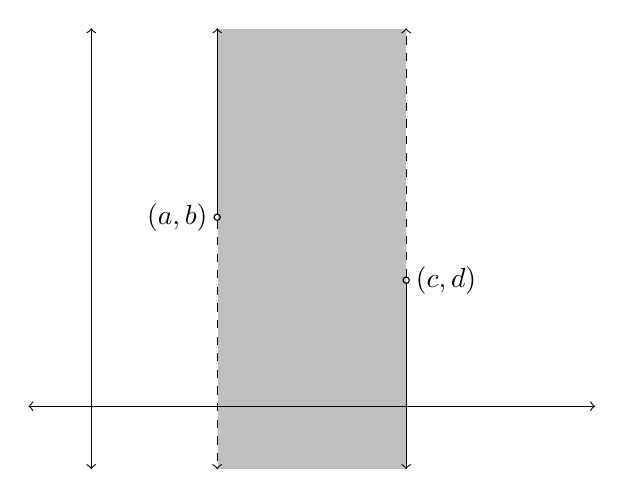
\begin{tikzpicture}[scale=0.8]
          \draw[white, fill=lightgray] (2,-1) rectangle (5,6);
          \draw[<->] (-1,0)--(8,0);
          \draw[<->] (0,-1)--(0,6);
          \draw[->] (2,3.05)--(2,6);
          \draw[->] (5,1.95)--(5,-1);
          \draw (2,3) circle [radius=0.05];
          \draw (5,2) circle [radius=0.05];
          \draw[dashed, ->] (2,2.95)--(2,-1);
          \draw[dashed,->] (5,2.05)--(5,6);
          \node[left] at (2,3) {$(a, b)$};
          \node[right] at (5,2) {$(c,d)$};
      \end{tikzpicture}
      \end{center}
    \end{example}

    \begin{example}
      The set of positive integers $\mathbb{Z}_+$ form an ordered set with a smallest element. The order topology for $\mathbb{Z}_+$ is precisely the discrete topology since every one-point set is an open set. 
      \[\{n\} = (n-1, n+1)\]
    \end{example}

    \begin{example}
      The dictionary order topology on $\{1, 2\} \times \mathbb{Z}_+$ results in every one point set being open, except for the point $(2, 1)$. Since every neighborhood of $(2,1)$ must contain some point of form $(1, n)$ for arbitrarily large $n$, $\{(2,1)\}$ is not open. 
    \end{example}

    \begin{definition}
      If $X$ is an ordered set a $a \in X$, then there are 4 subsets of $X$ called rays determined by $a$. 
      \begin{enumerate}
        \item $(a, +\infty)$ 
        \item $(-\infty, a)$
        \item $[a, +\infty)$
        \item $(-\infty, a]$
      \end{enumerate}
      The first two sets are called \textbf{open rays}, and the latter two sets are called \textbf{closed rays}. 
    \end{definition}

  \subsection{Quotient Topologies}

    \begin{definition}
    Let $X$ and $Y$ be topological spaces, and let $p: X \longrightarrow Y$ be a surjective map. The map $p$ is said to be a \textbf{quotient map} if
    \[U \text{ is open in } Y \iff p^{-1}(U) \text{ is open in } X\]
    \end{definition}

    Note that the conditions for being a quotient map is stronger then regular continuity. It is sometimes called \textbf{strong continuity}. An equivalent condition for $p$ to be a quotient map is to require that given $A \subset Y$, 
    \[A \text{ closed in } Y \iff p^{-1}(A) \text{ closed in } X\]
    This equivalence follows from the fact that
    \[f^{-1}(Y \setminus B) = X \setminus f^{-1}(B)\]

    \begin{definition}
    A subset $C \subset X$ is \textbf{saturated} with respect to the surjective map $p: X \longrightarrow Y$ if for every $p^{-1} (A)$ (where $A \subset Y$) that intersects $C$, $p^{-1}(A)$ is completely contained within $C$. That is, 
    \[p^{-1} \big( p(C) \big) = C\]
    \end{definition}

    In the visual below, we can see that $C_1$ and $C_2$ alone are not saturated, but $C_1 \cup C_2$ is saturated. Visually, for a given set $C \subset X$ to be saturated, there cannot be any points $q \not\in C$ such that $q \in p(C)$. 

    \begin{center}
    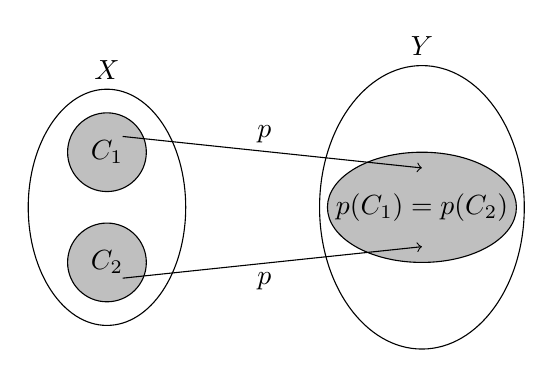
\begin{tikzpicture}
        \draw (0,0) ellipse (1 and 1.5);
        \draw[fill=lightgray] (0, 0.7) circle (0.5);
        \draw[fill=lightgray] (0, -0.7) circle (0.5);
        \node[above] at (0,1.5) {$X$};
        \draw (4,0) ellipse (1.3 and 1.8);
        \node[above] at (4,1.8) {$Y$};
        \draw[fill=lightgray] (4,0) ellipse (1.2 and 0.7);
        \node at (0, 0.7) {$C_1$};
        \node at (0,-0.7) {$C_2$};
        \node at (4,0) {$p(C_1) = p(C_2)$};
        \draw[->] (0.2,0.9)--(4,0.5);
        \draw[->] (0.2,-0.9)--(4,-0.5);
        \node[above] at (2, 0.7) {$p$};
        \node[below] at (2, -0.7) {$p$};
    \end{tikzpicture}
    \end{center}
    We now introduce an alternative, equivalent definition of quotient maps. 

    \begin{definition}
    $p: X \longrightarrow Y$ is a quotient map if and only if $p$ is continuous and $p$ maps saturated open sets of $X$ to open sets of $Y$ (or saturated closed sets of $X$ to closed sets of $Y$). 
    \end{definition}

    \begin{proposition}
    If $p: X \longrightarrow Y$ is a surjective, continuous map that is either open or closed (that is, maps open sets to open sets or closed sets to closed sets), then $p$ is a quotient map. 

    Note however, that the converse is not true; there exists quotient maps that are neither open nor closed. 
    \end{proposition}

    \begin{definition}
    If $X$ is a space and $A$ is a set and if $p: X \longrightarrow A$ is a surjective map, then there exists exactly one topology $\mathscr{T}$ on $A$ relative to which $p$ is a quotient map. $\mathscr{T}$ is called the \textbf{quotient topology} induced by $p$. 
    \end{definition}

    To construct the quotient topology for the surjective map $p$, we must make $p$ continuous. Therfore, the topology $\mathscr{T}$ on $A$ is defined by letting it consist of all subsets $U$ of $A$ such that $p^{-1}(U)$ is open in $X$. This is indeed a topology since
    \begin{enumerate}
        \item $p^{-1} (\emptyset) = \emptyset$ and $p^{-1}(A) = X$
        \item $p^{-1} \Big( \bigcup_{\alpha \in J} U_\alpha \Big) = \bigcup_{\alpha \in J} p^{-1} (U_\alpha)$
        \item $p^{-1} \Big( \bigcap_{i=1}^n U_i \Big) = \bigcap_{i=1}^n p^{-1} (U_i)$
    \end{enumerate}

    We can also construct the quotient topology as the final topology. 

    \begin{definition}
    Given a mapping 
    \[f: (X, \tau_X) \longrightarrow (Y, \tau_Y)\]
    where $\tau_X$ is well-defind and $\tau_Y$ is not, the finest possible topology available on $Y$ that makes $f$ continuous is called the \textbf{final topology of $Y$}. 
    \end{definition}

    Note that we say the "finest possible topology" when defining the final topology. It is because if $\tau_Y$ is too fine (e.g. if $\tau_Y = 2^Y$), then the open sets of $\tau_Y$ would be too fine and therefore would have a preimage that may not be open in $X$. 

    \begin{example}
    Let $p: (\mathbb{R}, \tau_\mathbb{R}) \longrightarrow \mathbb{R} / 2 \pi \mathbb{R}$. Then, the final topology of $\mathbb{R} / 2 \pi \mathbb{R}$ would be simply defined 
    \[\tau_{\mathbb{R} / 2 \pi \mathbb{R}} \equiv \{U \subset \mathbb{R} / 2\pi \mathbb{R} \; | \; U = p(O), O \in \tau_\mathbb{R}\}\]
    That is, the quotient topology is merely the set of all images of open sets in $\mathbb{R}$ under $f$. However, if $\mathbb{R} / 2 \pi \mathbb{R}$ has the discrete topology $2^X$, then a single equivalence class, say $[0]$, will get mapped to the collection of points $\{2 \pi k \; | \; k \in \mathbb{Z}\}$, which is clearly not open in $\mathbb{R}$. Note that the final topology (or the quotient topology) is endowed onto the codomain in order to make $f$ continuous (or a quotient mapping). 
    \end{example}

    \begin{proposition}
    Given a relation $\sim$ on a topological space $(X, \tau_X)$, the quotient topology of the quotient space $X / \sim$, is precisely the final topology on the quotient set with respect to the quotient map $p: X \longrightarrow X / \sim$. That is, 
    \[\tau_{X / \sim} \equiv \big\{U \subseteq X / \sim \; | \; \{x \in X \; | \; p(x) \in U\} \in \tau_X \big\}\]
    which is the topology whose open sets are the subsets of $X / \sim$ that have an open preimage under the surjective map $p: x \mapsto [x]$. 
    \end{proposition}

    \begin{example}
    Let $X \equiv [0,1] \cap [2,3] \subset \mathbb{R}$ and $Y y \equiv [0,2] \subset \mathbb{R}$. Then, we define $p: X \longrightarrow Y$ as 
    \[p(x) \equiv \begin{cases}
          x & x \in [0,1] \\
          x-1 & x \in [2,3]
    \end{cases}\]
    $p$ is continuous (under subspace topology of $X \subset \mathbb{R}$), surjective, and closed, meaning that it is a quotient map. However, it is not open, since the image of the open set $[0,1]$ of $X$ is $[0,1]$, which is not open in $Y$. 
    \end{example}

    \begin{example}
    Let $p: \mathbb{R} \longrightarrow \{a, b, c\}$ be defined as 
    \[p(x) \equiv \begin{cases}
          a & x > 0 \\
          b & x < 0 \\
          c & x = 0
    \end{cases}\]
    Then, the quotient topology of $\{a, b, c\}$ consists of 
    \[\emptyset, \{a\}, \{b\}, \{a, b\}, \{a, b, c\}\]
    \end{example}

    \begin{definition}
    Let $X$ be a topological space, and let $\Tilde{X}$ be a partition of $X$ into disjoint subsets whose union is $X$. Let $p: X \longrightarrow \Tilde{X}$ be the surjective map mapping every point $x \in X$ to the subset that it is in. In the quotient topology induced by $p$, $\Tilde{X}$ is called the quotient space of $X$. 
    \end{definition}

    To construct a quotient space, we can equivalently define a relation on $X$. That is, a subset $U$ of $\Tilde{X}$ is a collection of equivalence classes, and the set $p^{-1}(U)$ is the union of equivalence classes belonging to $U$. Therefore, the typical open set of $\Tilde{X}$ is a collection of equivalence classes whose union is an open set in $X$. 

    \begin{example}[Construction of a Torus]
    Let $X \equiv [0,1] \times [0,1] \subset \mathbb{R}^2$. We define an equivalence relation $Y$ consisting of the equivalence classes
    \begin{align*}
        &\big\{\{(x, y)\} \; | \; 0<x, y<1\big\} \cup \big\{ \{(x, 0), (x,1)\} \; | \; 0<x<1 \big\} \cup \\
        &\big\{ \{(0,y), (1,y)\} \; | \; 0<y<1 \big\} \cup \big\{ \{(0,0), (0,1), (1,0), (1,1)\} \big\}
    \end{align*}
    Then, the quotient topology of this quotient space consists of open sets of form
    \begin{center}
    \begin{tikzpicture}
        \draw (0,0) rectangle (2,2);
        \draw (3,0) rectangle (5,2);
        \draw (6,0) rectangle (8,2);
        \draw (9,0) rectangle (11,2);
        \draw[dashed] (1, 1.5) circle [radius=0.4];
        \draw[fill] (1, 1.5) circle [radius=0.03];
        \draw[dashed] (3.9,0) arc (0:180: 0.4);
        \draw[dashed] (3.9,2) arc (0:-180:0.4);
        \draw[dashed] (6,1.1) arc (-90:90:0.4);
        \draw[dashed] (8,1.9) arc (90:270:0.4);
        \draw[fill] (3.5,0) circle [radius=0.03];
        \draw[fill] (3.5,2) circle [radius=0.03];
        \draw[fill] (6,1.5) circle [radius=0.03];
        \draw[fill] (8,1.5) circle [radius=0.03];
        \draw[fill] (9,0) circle [radius=0.03];
        \draw[fill] (11,0) circle [radius=0.03];
        \draw[fill] (9,2) circle [radius=0.03];
        \draw[fill] (11,2) circle [radius=0.03];
        \draw[dashed] (9.4,0) arc (0:90:0.4);
        \draw[dashed] (9.4,2) arc (0:-90:0.4);
        \draw[dashed] (11,0.4) arc (90:180:0.4);
        \draw[dashed] (10.6,2) arc (180:270:0.4);
    \end{tikzpicture}
    \end{center}
    This quotient space $X / Y$ is homeomorphic to the torus $S^1 \times S^1$, denoted
    \[\frac{X}{Y} \cong S^1 \times S^1\]
    We can visualize the construction of the equivalence relation $Y$ as a "gluing" of the rectangle $X$ by its edges and corners. 

    We can check that this mapping is indeed a quotient map. First, it is clearly surjective. By realizing that individual points on the edge of $[0,1]^2$ are open sets themselves (by the subspace topology), we can prove that this map is indeed open and continuous. 
    \end{example}

    \begin{example}[Construction of the 2-Sphere]
    Let $X$ be the closed unit ball 
    \[X \equiv \{(x, y) \in \mathbb{R}^2 \; | \; x^2 + y^2 \leq 1\}\]
    and define the equialence classes $R$ as 
    \[R \equiv \big\{ \{(x, y)\} \; | \; x^2 + y^2 <1 \big\} \cup \{S^1\}\]
    which will consist of open sets of one of the two forms
    \begin{center}
    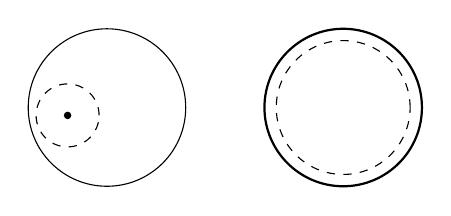
\begin{tikzpicture}
        \draw (1,1) circle [radius=1];
        \draw[thick] (4,1) circle [radius=1];
        \draw[dashed] (0.5,0.9) circle [radius=0.4];
        \draw[fill] (0.5,0.9) circle [radius=0.04];
        \draw[dashed] (4,1) circle [radius=0.85];
    \end{tikzpicture}
    \end{center}
    Then, this quotient space $X / R$ is homeomorphic to the 2-sphere
    \[S^2 \equiv \{(x, y, z) \in \mathbb{R}^3 \; | \; x^2 + y^2 + z^2 = 1\}\]
    Visually, we can imagine the disk being glued together by its sides to continuously form the 2-sphere. 
    \end{example}

    \begin{example}[Construction of the 1-Sphere]
    We will show that
    \[\frac{\mathbb{R}}{\mathbb{Z}} \cong S^1\]
    Let us construct the set $(\mathbb{R}, \tau_{\mathbb{R}})$ with paramater $t$. We define maps
    \begin{align*}
    p: \mathbb{R} \longrightarrow \mathbb{R} / \mathbb{Z}, \;\; p(t) \equiv t \; (\text{mod } 1) \\
    q: \mathbb[R] \longrightarrow S^1 \subset \mathbb{C}, \;\; g(t) \equiv e^{2 \pi i t} 
    \end{align*}
    We claim that $p$ and $q$ are both quotient mappings. Clearly, $p$ is a quotient mapping. As for $q$, it it easy to see that it is surjective (but not injective) and continuous ($\tau_{S^1}$ has the basis of open intervals on $S^1$). It is also easy to notice that given an open interval $U \subset S^1$, $q^{-1}(U)$ will be the union of open intervals equally spaced in $\mathbb{R}$. Additionally, given any open interval in $\mathbb{R}$, it maps to an open interval in $S^1$ (note that $S^1$ itself is also open). These three conditions imply that $q$ is a quotient map. We now define maps 
    \[ q \circ p^{-1}: \mathbb{R} / \mathbb{Z} \longrightarrow S^1 \]
    \[ p \circ q^{-1}: S^1 \longrightarrow \mathbb{R} / \mathbb{Z} \]
    and claim that these maps are homeomorphisms. We can clearly see that the mapping from an open set in $\mathbb{R} / \mathbb{Z}$ to the union of spaced open intervals in $\mathbb{R}$ is an injection, and the mapping from this union of open intervals to the union of open intervals in $S^1$ is a surjection. The composition of these two mappings clearly defines a bijection. Therefore, $q \circ p^{-1}$ is proven to be a bicontinuous bijective mapping between open sets $U \subset \mathbb{R} / \mathbb{Z}$ and $V \subset S^1 \implies$ $q \circ p^{-1}$ is a homeomorphism. 

    This result clearly makes sense since 
    \[\frac{\mathbb{R}}{\mathbb{Z}} \cong \frac{[0,1]}{\sim}\]
    where the relation $\sim$ maps every point $x \in (0,1)$ to its own equivalence class and the points $0, 1$ to one equivalence class $\{0\}$. Therefore, it is informally said that the quotient space of the real line is a circle. 

    One may attempt to construct a simpler set by replacing $S^1$ with the half-open interval $[0,1)$. However, while $[0,1)$ is bijective to $\mathbb{R} / \mathbb{Z}$,
    \[\frac{\mathbb{R}}{\mathbb{Z}} \not\cong [0,1)\]
    That is, the two sets are not homeomorphic because the topologies of $[0,1)$ and $\mathbb{R} / \mathbb{Z}$ are not compatible. For instance, when we attempt to map the open set 
    \[ \bigg\{ [x] \in \mathbb{R} / \mathbb{Z} \; | \; 0 \leq x \leq \frac{1}{4} \vee x > \frac{1}{2} \bigg\} \in \tau_{\mathbb{R} / \mathbb{Z}} \]
    to $\tau_{[0,1)}$, it does not return an open set. 


    Furthermore, this means that
    \[S^1 \times S^1 \cong \frac{[0,1]^2}{\sim^\prime} \cong \bigg( \frac{\mathbb{R}}{\mathbb{Z}} \bigg)^2\]
    where $\sim^\prime$ is the quotient mapping defined in the previous construction of the torus. 
    \end{example}

    \begin{example}[Construction of the Cylinder]
    Let us define the cylinder as 
    \[C \equiv \{(x, y, z) \in \mathbb{R}^3 \; | \; x^2 + y^2 = 1, z \in [0,1]\} \]
    Then, we can see that
    \[C \cong \frac{[0,1]^2}{\sim}\]
    where $\sim$ is the equivalence relation defined by the quotient mapping 
    \[p\big((x, y)\big) \equiv \begin{cases}
          \{(x, y)\} & x \neq 0, x \neq 1 \\
          \{(0,y), (1, y)\} & x = 0 \text{ or } x = 1
    \end{cases}\]
    \end{example}

    Subspaces do not behave well under quotient maps. That is, if $p: X \longrightarrow Y$ is a quotient map and $A$ is a subspace of $X$, then the map $p^\prime: A \longrightarrow p(A)$ obtained by restricting both the domain and codomain of $P$ need not be a quotient map. Additionally, quotient maps are clearly not homeomorphisms, so topological properties are not preserved. 

    However, composites of maps do behave nicely. 

    \begin{proposition}
    The composition of two quotient maps is a quotient map. 
    \end{proposition}
    \begin{proof}
    Indeed, the composition of surjective, continuous, and open maps is surjective, continuous, and open. 
    \end{proof}

    However, the product of two quotient maps is not necessarily a quotient map. That is, given $p: A \longrightarrow B$ and $q: C \longrightarrow D$ are quotient maps, the map 
    \[p \times q: A \times C \longrightarrow B \times D, \; (p \times q) (a \times c) \equiv p(a) \times q(c)\]
    is not necessarily a quotient map. 

    \begin{example}
    Given $(\mathbb{R}, \tau_{\mathbb{R}})$, let us define the relation $\sim$ determined by the quotient mapping
    \[p(x) \equiv \begin{cases}
          \{x\} & x \not\in \mathbb{Z} \\
          \mathbb{Z} & x \in \mathbb{Z}
    \end{cases}\]
    In words, this quotient map maps every integer to the equivalence class $[0]$ and maps every other point to its own class. It turns out that every interval $[j, j+1] \subset \mathbb{R}, \; j \in \mathbb{Z}$ will get mapped as a closed loop in $\mathbb{R} / \sim$ beginning and ending with $[0]$, since $j, j+1 \mapsto [0]$. So geometrically, $\mathbb{R} / \sim$ consists of an infinite number of nonintersecting closed loops starting and ending with $[0]$. 
    \begin{center}
    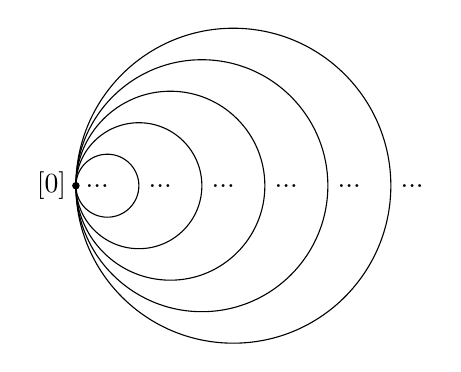
\begin{tikzpicture}[scale=0.4]
        \draw (5,0) circle (5);
        \node[left] at (0,0) {$[0]$};
        \draw[fill] (0,0) circle (0.1);
        \draw (4,0) circle (4);
        \draw (3,0) circle (3);
        \draw (2,0) circle (2);
        \draw (1,0) circle (1);
        \node[right] at (0,0) {...};
        \node[right] at (2,0) {...};
        \node[right] at (4,0) {...};
        \node[right] at (6,0) {...};
        \node[right] at (8,0) {...};
        \node[right] at (10,0) {...};
    \end{tikzpicture}
    \end{center}

    This wacky mapping is an example of a quotient mapping that does not preserve topological structure. While it will not be proven here, it is known that $(\mathbb{R}, \tau_{\mathbb{R}})$ is 1st and 2nd countable, but $\mathbb{R} / \sim$ under this relation is not even 1st countable. 
    \end{example}

    We now introduce theorems of continuous maps from quotient spaces inducing other continuous maps. 

    \begin{theorem}
    Let $p: (X, \tau_X) \longrightarrow (Y, \tau_Y)$ be a quotient map. Let $(Z, \tau_Z)$ be a topological space and let there exist a function $f: Y \longrightarrow Z$. $f$ is continuous if and only if $f \circ p$ is continuous. 
    \[\begin{tikzcd}
        X \arrow{d}{p} \arrow{rd}{f \circ p}\\
        Y \arrow{r}{f} & Z
    \end{tikzcd}\]
    \end{theorem}
    \begin{proof}
    ($\rightarrow$) Assume $f$ is continuous. By definition of the quotient topology, $p$ is continuous $\implies$ $f \circ p$ is continuous. \\
    ($\leftarrow$) Assume $f \circ p$ is continuous $\iff (f \circ p)^{-1} (\omega) \in \tau_X$ for every $\omega \in \tau_Z \iff p^{-1} \big( f^{-1}(\omega) \big) \in \tau_X$, but $p$ is continuous, so $f^{-1}(\omega)$ is open in $Y$. Therefore, given $\omega \in \tau_{Z}$, $f^{-1} (\omega) \in \tau_Y \implies f$ is continuous. 
    \end{proof}

    The previous theorem determines continuity of $f$ and $f \circ p$ given a function mapping $Y \longrightarrow Z$. The following analogous theorem determines continuity of an induced map $f$ given a function mapping $X \longrightarrow Z$. 

    \begin{theorem}
    Let $p: (X, \tau_X )\longrightarrow (Y, \tau_Y)$ be a quotient map. Let $Z$ be a space and let $g: X \longrightarrow Z$ be a map such that $g$ is constant on the elements $x$ of each equivalence class induced by $p$. That is, if $x_1$ and $x_2$ are in the same equivalence class induced by $p$, i.e. 
    \[p(x_1) = p(x_2)\]
    then $g(x_1) = g(x_2)$. If $g$ is continuous, then $g$ induces a continuous map $f: X \longrightarrow Z$ such that $g = f \circ p$. That is, 
    the diagram below commutes 
    \[\begin{tikzcd}
        X \arrow{d}{p} \arrow{rd}{g=f \circ p}\\
        Y \arrow{r}{f} & Z
    \end{tikzcd}\]
    \end{theorem}

